\documentclass[sigconf,nonacm,screen]{acmart}
\usepackage{filecontents}
\usepackage{textcomp}
\usepackage{pgfplots}
\usetikzlibrary{patterns}
\usepackage{ifthen}
\usepgfplotslibrary{groupplots}
\RequirePackage{keyval}
\usepackage{multirow}
\usepackage{multicol}
\usepackage{csvsimple}
\usepackage[utf8]{inputenc}
\newcounter{row}
\newcounter{col}
\usepackage{wrapfig}
\usepackage{textgreek}
\usepackage[inline]{enumitem}
% \usepackage[table]{xcolor}
\usetikzlibrary{matrix, positioning}
\usetikzlibrary{patterns,tikzmark}
\usetikzlibrary{matrix,decorations.pathreplacing,calc}
\usepackage{hf-tikz}
\usepackage{pifont}
\usepackage{subfig}
\usetikzlibrary{chains,fit,shapes}
\usetikzlibrary{arrows.meta,
    chains,
    positioning,
    shapes.symbols}
\usetikzlibrary{decorations,calligraphy}
\usepackage{pgfplotstable}
\usepgfplotslibrary{statistics}
%\pgfplotsset{compat=newest}
\usetikzlibrary{matrix,calc}
\usetikzlibrary{fit}
\usepackage{xfp}
\usepackage{mathtools}

\usetikzlibrary{positioning}

\usepackage{makecell}
%\usepackage{tabu}
\usepackage{tikz}
\usetikzlibrary{trees}

%\pgfplotsset{compat=1.8}
\pgfplotsset{compat=1.12}


\usepgfplotslibrary{fillbetween}

\usepackage{filecontents}
% \usetikzlibrary{pgfplots.groupplots}
% \pgfplotsset{compat=1.9}

% \usepackage[utf8]{inputenc}
% \usepackage[ngerman]{babel}
% \usepackage{pgfplots}
% \pgfplotsset{compat=1.9}
% \usetikzlibrary{
%   pgfplots.groupplots,
%   matrix
% }
% \usepackage{siunitx}

\newtheorem{theorem}{Theorem}
\newtheorem{definition}{Definition}
\newcommand{\eat}[1]{}

\definecolor{bluegreen}{RGB}{3, 166, 155}
\definecolor{pitchblack}{RGB}{0, 0, 0}
\definecolor{lightbeige}{RGB}{255, 251, 241}
\definecolor{mediumgray}{RGB}{183, 183, 183}
\definecolor{mygreen}{rgb}{0,0.6,0}
\definecolor{mygray}{rgb}{0.5,0.5,0.5}
\definecolor{mymauve}{rgb}{0.58,0,0.82}
\definecolor{keywords}{RGB}{255,0,90}
\definecolor{comments}{RGB}{0,0,113}
\definecolor{red}{RGB}{255,0,0}
\definecolor{green}{RGB}{0,255,0}
\definecolor{navy}{RGB}{0,0,128}
\definecolor{DarkGrenen}{RGB}{0,100,0}
\definecolor{DarkOliveGreen}{RGB}{85,107,47}
\definecolor{saddlebrown}{RGB}{139,69,19}
\definecolor{gold}{RGB}{252,194,1}
\definecolor{tug}{RGB}{247,1,70}
\definecolor{tugb}{RGB}{120,137,251}

\definecolor{color01}{RGB}{159,96,0}
\definecolor{color02}{RGB}{43,85,128}


\definecolor{blue0}{RGB}{153,153,153}
\definecolor{blue1}{RGB}{77,77,77}%
\definecolor{blue2}{RGB}{165,71,209}
\definecolor{blue3}{RGB}{77,10,142}
\definecolor{blue4}{RGB}{74,139,203}
\definecolor{blue5}{RGB}{40,40,190}

\definecolor{color1}{RGB}{100,149,237} % corn flower blue
\definecolor{color2}{RGB}{153,153,153} % light gray
\definecolor{color3}{RGB}{0,0,0} % black
\definecolor{color4}{RGB}{255,165,0} % orange
\definecolor{color5}{RGB}{255,69,0} % orange red
\definecolor{color6}{RGB}{77,77,77} % dark gray
\definecolor{color7}{RGB}{31,119,180}
\definecolor{color8}{RGB}{7,77,125}
\definecolor{color9}{RGB}{153,216,201}


\definecolor{teal1}{RGB}{31, 111, 111}
\definecolor{teal2}{RGB}{84, 161, 161}
\definecolor{teal3}{RGB}{159, 200, 200}

\definecolor{dred1}{RGB}{160, 0, 0}
\definecolor{dred2}{RGB}{196, 102, 102}
\definecolor{dred3}{RGB}{216, 166, 166}


\definecolor{dblue1}{RGB}{32, 102, 168}
\definecolor{dblue2}{RGB}{53, 148, 204}
\definecolor{dblue3}{RGB}{140, 197, 227}

\definecolor{totalcolor}{RGB}{2, 152, 215}
\definecolor{mvcolor}{RGB}{248, 163, 47}
\definecolor{dvcolor}{RGB}{203, 70, 39}



% Enable this two commands when you want to extract diagrams in extra files, then run "make"
\usetikzlibrary{external}
\tikzexternalize[prefix=plots/] %  activate

\usetikzlibrary{positioning}

\sloppy
\clubpenalty = 10000
\widowpenalty = 10000
\brokenpenalty = 10000
\frenchspacing


\makeatletter
\def\pgfplots@drawaxis@lines@preparediscont@for#1{%
        \ifnum\csname pgfplots@#1axisdiscontnum\endcsname>0
                \begingroup
                % this group employs several temporary dimension registers
                % and is therefor scoped:
                \let\disstart=\pgf@ya
                \let\disend=\pgf@yb
                \disend=\csname pgfplots@#1max@reg\endcsname
                \advance\disend by -\csname pgfplots@#1min@reg\endcsname
                \disend=\csname pgfplots@#1@veclength\endcsname\disend
                \ifcase\csname pgfplots@#1axisdiscontnum\endcsname\relax
                        % has already been checked above.
                \or
                        \def\discontstyle{decoration={zigzag,segment length=5pt, amplitude=2pt}}%
                        \advance \disend by -8pt
                \or
                        \def\discontstyle{decoration={ticks,segment length=4pt, amplitude=8pt}}%
                        \advance \disend by -4pt
                \fi
                \pgfplotscoordmath{#1}{datascaletrafo get params}%
                % if #1max + shift < 0pt  (shift is 0 without the scaling trafo)
                \ifdim\csname pgfplots@#1max@reg\endcsname<-\pgfplotsretvalb pt
                        % swap start and end
                        \disstart=\disend
                        \disend=2pt
                \else
                        \disstart=2pt
                \fi
                % carry local computations outside of group:
                \xdef\pgfplots@glob@TMPa{%
                        \noexpand\def\expandafter\noexpand\csname #1disstart\endcsname{\the\disstart}%
                        \noexpand\def\expandafter\noexpand\csname #1disend\endcsname{\the\disend}%
                        \noexpand\pgfkeysdef{/tikz/#1discont}{\noexpand\pgfkeysalso{\discontstyle}}%
                }%
                \endgroup
                \pgfplots@glob@TMPa
        \else
                \expandafter\def\csname #1disstart\endcsname{0pt}%
                \expandafter\def\csname #1disend\endcsname{0pt}%
                \pgfkeyslet{/tikz/#1discont}=\pgfutil@empty
        \fi
}%
\makeatother



\begin{document}
\title[Query Processing by Data Catalog]{Query Processing by Data Catalog}

\author{Saeed Fathollahzadeh} 
\orcid{0000-0003-3723-6191}
\affiliation{
\institution{Concordia University}
\country{Canada}}

\renewcommand{\shortauthors}{Saeed Fathollahzadeh}

\maketitle


    % \tikzsetnextfilename{Experiment1-Micro-Tic-Tac-Toe} 
    %     \begin{figure}[!ht]
    %         \centering
    %         \makeatletter
\newcommand\resetstackedplots{
\makeatletter
\pgfplots@stacked@isfirstplottrue
\makeatother
\addplot [forget plot,draw=none] coordinates{(gemini-1.5-pro-latest, 0) (llama3-70b-8192, 0) (gpt-4o, 0)};
}
\makeatother

\begin{tikzpicture}

   \newcommand{\myaddplotauc}[6]{ 
      \addplot[xshift=#6,fill=#5, draw=black,line width=0.3pt] 
      table[y=test_auc, col sep=comma, x=llm_model, discard if singlconfig={No}{#1}{#2}{#3}{#4}]%, 
      {../archive/SIGMOD2025-Results/MicroResults.csv};
      \label{#2}       
    };

    \newcommand{\myaddplotdsg}[6]{
      \resetstackedplots
      \myaddplotauc{#1}{SDVC}{#2}{0}{dred3}{#3};
      \resetstackedplots
      \myaddplotauc{#1}{S}{#2}{0}{dred2}{#4};
      \resetstackedplots
      \myaddplotauc{#1}{SCV}{#2}{0}{dred1}{#5};
      \resetstackedplots
      \myaddplotauc{#1}{CatDBChain}{#2}{0}{dblue1}{#6};
    };

    \pgfplotsset{
      discard if singlconfig/.style n args={5}{
          x filter/.code={
              \edef\tempa{\thisrow{has_description}}
              \edef\tempb{#1}
              \ifx\tempa\tempb
                \edef\tempc{\thisrow{llm_model}}
                  \edef\tempd{#2}
                    \ifx\tempc\tempd  
                    %
                      \edef\tempe{\thisrow{config}}
                      \edef\tempf{#3}
                      \ifx\tempe\tempf  
                      %
                        \edef\tempg{\thisrow{dataset_name}}
                        \edef\temph{#4}
                        \ifx\tempg\temph
                        
                          \edef\tempi{\thisrow{number_of_samples}}
                          \edef\tempj{#5}
                          \ifx\tempi\tempj                                      
                          \else
                          \def\pgfmathresult{inf}
                          \fi
                             
                        \else
                        \def\pgfmathresult{inf}
                        \fi
                    %           
                      \else
                      \def\pgfmathresult{inf}
                    \fi
                    %                
                    \else
                    \def\pgfmathresult{inf}
                    \fi
              \else
              \def\pgfmathresult{inf}
              \fi			
          }
      },
  };   

\begin{axis}[
  ybar stacked,
  ymin=0,
  ymax=1,
  y tick label style={/pgf/number format/1000 sep={}},
  x tick label style={/pgf/number format/1000 sep={}},  
  scaled y ticks=false,
  axis line style={black, line width=0.3pt},
  enlarge y limits={0.3,upper},
  enlarge x limits=0.07,
  ylabel={Test AUC $\%$},
  xlabel={},
  log ticks with fixed point,
  xtick align=outside,
  xtick pos=left,
  ytick pos=left,
  yticklabel style = {font=\normalsize},
  ylabel style = {font=\normalsize, yshift=-3pt, xshift=-3pt},
  height=.5\columnwidth,
  width=0.8\columnwidth,
  ymajorgrids=true,
  grid style=dotted,
  minor grid style={gray!70},
  every axis plot/.append style={line width=0.4pt,mark options={scale=1.5,solid}},  
  xticklabel style = {font=\normalsize, xshift=0pt, yshift=3pt},
  legend image post style={line width=.5pt},          
  bar width=8pt,         
  ytick={0,0.2,0.4,0.6,0.8,1},
  yticklabels={0, 20, 40, 60, 80, 100},               
  every x tick/.style={ draw=none},
  xtick = data,
  symbolic x coords={gemini-1.5-pro-latest, llama3-70b-8192, gpt-4o},
  xticklabels={\hspace{0.8cm}Gemini-1.5, \hspace{0.1cm}Llama3-70b, \hspace{-0.64cm}GPT-4o},
  legend image code/.code={\draw [#1] (0cm,-0.08cm) rectangle (0.15cm,0.08cm); }, 
]
\myaddplotdsg{gpt-4o}{Tic-Tac-Toe}{-24pt}{-16pt}{-8pt}{0pt}
\myaddplotdsg{gemini-1.5-pro-latest}{Tic-Tac-Toe}{0pt}{8pt}{16pt}{24pt}
\myaddplotdsg{llama3-70b-8192}{Tic-Tac-Toe}{-15pt}{-7pt}{1pt}{9pt}

\end{axis}

\node [draw=none,inner sep=0, font=\scriptsize, anchor=west] (leg1) at (rel axis cs: 0.1,0.9) {\shortstack[l]{
  \ref{SDVC} Schema + Distinct Value Count \\ 
  \ref{SCV} Schema + Categorical Values}};

  \node [draw=none,inner sep=0, font=\scriptsize, anchor=west, right=of leg1, xshift=-13pt]  {\shortstack[l]{
   \ref{S} Schema \\ 
   \ref{CatDBChain} CatDB Chain
  }};

\end{tikzpicture}
    %         \caption{Experiment1-Micro-Tic-Tac-Toe}
    %     \end{figure}  

    % \tikzsetnextfilename{Experiment1-Micro-Walking-Activity} 
    %     \begin{figure}[!ht]
    %         \centering
    %         \makeatletter
\newcommand\resetstackedplots{
\makeatletter
\pgfplots@stacked@isfirstplottrue
\makeatother
\addplot [forget plot,draw=none] coordinates{(gemini-1.5-pro-latest, 0) (llama3-70b-8192, 0) (gpt-4o, 0)};
}
\makeatother

\begin{tikzpicture}

   \newcommand{\myaddplotauc}[6]{ 
      \addplot[xshift=#6,fill=#5, draw=black,line width=0.3pt] 
      table[y=test_auc_ovr, col sep=comma, x=llm_model, discard if singlconfig={No}{#1}{#2}{#3}{#4}]%, 
      {../archive/SIGMOD2025-Results/MicroResults.csv};
      \label{#2}       
    };

    \newcommand{\myaddplotdsg}[8]{
      \resetstackedplots
      \myaddplotauc{#1}{S}{#2}{0}{white}{#3};
      \resetstackedplots
      \myaddplotauc{#1}{SDVC}{#2}{0}{dred1!10}{#4};
      \resetstackedplots
      \myaddplotauc{#1}{SSN}{#2}{0}{dred1!35}{#5};
      \resetstackedplots
      \myaddplotauc{#1}{SCV}{#2}{0}{dred1!60}{#6};
      \resetstackedplots
      \myaddplotauc{#1}{SDVCSN}{#2}{0}{dred1}{#7};      
      \resetstackedplots
      \myaddplotauc{#1}{CatDBChain}{#2}{0}{dblue1}{#8};
    };

    \pgfplotsset{
      discard if singlconfig/.style n args={5}{
          x filter/.code={
              \edef\tempa{\thisrow{has_description}}
              \edef\tempb{#1}
              \ifx\tempa\tempb
                \edef\tempc{\thisrow{llm_model}}
                  \edef\tempd{#2}
                    \ifx\tempc\tempd  
                    %
                      \edef\tempe{\thisrow{config}}
                      \edef\tempf{#3}
                      \ifx\tempe\tempf  
                      %
                        \edef\tempg{\thisrow{dataset_name}}
                        \edef\temph{#4}
                        \ifx\tempg\temph
                        
                          \edef\tempi{\thisrow{number_of_samples}}
                          \edef\tempj{#5}
                          \ifx\tempi\tempj                                      
                          \else
                          \def\pgfmathresult{inf}
                          \fi
                             
                        \else
                        \def\pgfmathresult{inf}
                        \fi
                    %           
                      \else
                      \def\pgfmathresult{inf}
                    \fi
                    %                
                    \else
                    \def\pgfmathresult{inf}
                    \fi
              \else
              \def\pgfmathresult{inf}
              \fi			
          }
      },
  };   

\begin{axis}[
  ybar stacked,
  ymin=0,
  ymax=1,
  y tick label style={/pgf/number format/1000 sep={}},
  x tick label style={/pgf/number format/1000 sep={}},  
  scaled y ticks=false,
  axis line style={black, line width=0.3pt},
  enlarge y limits={0.42,upper},
  enlarge x limits=0.07,
  ylabel={Test AUC-ovr $\%$},
  xlabel={},
  log ticks with fixed point,
  xtick align=outside,
  xtick pos=left,
  ytick pos=left,
  yticklabel style = {font=\normalsize},
  ylabel style = {font=\normalsize, yshift=-3pt, xshift=-3pt},
  height=.5\columnwidth,
  width=1.27\columnwidth,
  ymajorgrids=true,
  grid style=dotted,
  minor grid style={gray!70},
  every axis plot/.append style={line width=0.4pt,mark options={scale=1.5,solid}},  
  xticklabel style = {font=\normalsize, xshift=0pt, yshift=3pt},
  legend image post style={line width=.5pt},          
  bar width=8pt,         
  ytick={0,0.2,0.4,0.6,0.8,1},
  yticklabels={0, 20, 40, 60, 80, 100},               
  every x tick/.style={ draw=none},
  xtick = data,
  symbolic x coords={gemini-1.5-pro-latest, llama3-70b-8192, gpt-4o},
  xticklabels={\hspace{1cm}Gemini-1.5, \hspace{-.8cm}Llama3-70b, \hspace{-1cm}GPT-4o},
  legend image code/.code={\draw [#1] (0cm,-0.1cm) rectangle (0.15cm,0.1cm); }, 
]
\myaddplotdsg{gpt-4o}{Walking-Activity}{-40pt}{-32pt}{-24pt}{-16pt}{-8pt}{0pt}
\myaddplotdsg{llama3-70b-8192}{Walking-Activity}{-28pt}{-20pt}{-12pt}{-4pt}{4pt}{12pt}
\myaddplotdsg{gemini-1.5-pro-latest}{Walking-Activity}{-4pt}{4pt}{12pt}{20pt}{28pt}{36pt}
\end{axis}

\node [draw=none,inner sep=0, font=\footnotesize, anchor=west] (leg1) at (rel axis cs: 0.065,0.86) {\shortstack[l]{
  \ref{S} Schema \ \ \ref{SDVC} Schema+Unique Count \ \ \ref{SSN} Schema+Statistical Numbers \ \ \ref{CatDBChain} CatDB Chain\\ 
  \ref{SCV} Schema+Categorical Values \ \ \ref{SDVCSN}  Schema+Unique Count+Statistical Numbers 
  }};

  % \node [draw=none,inner sep=0, font=\footnotesize, anchor=west, right=of leg1, xshift=-27pt] (leg2)  {\shortstack[l]{
    
    
  %   }};  

\end{tikzpicture}
    %         \caption{Experiment1-Micro-Walking-Activity}
    %     \end{figure}    
        
    \tikzsetnextfilename{Experiment1-Micro-Bike-Sharing} 
        \begin{figure}[!ht]
            \centering
            \makeatletter
\newcommand\resetstackedplots{
\makeatletter
\pgfplots@stacked@isfirstplottrue
\makeatother
\addplot [forget plot,draw=none] coordinates{(gemini-1.5-pro-latest, 0) (llama3-70b-8192, 0) (gpt-4o, 0)};
}
\makeatother

\begin{tikzpicture}

   \newcommand{\myaddplotauc}[6]{ 
      \addplot[xshift=#6,fill=#5, draw=black,line width=0.3pt] 
      table[y=test_r_squared, col sep=comma, x=llm_model, discard if singlconfig={No}{#1}{#2}{#3}{#4}]%, 
      {../archive/SIGMOD2025-Results/MicroResults.csv};
      \label{#2}       
    };

    \newcommand{\myaddplotdsg}[8]{
      \resetstackedplots
      \myaddplotauc{#1}{SSN}{#2}{0}{white}{#3};
      \resetstackedplots
      \myaddplotauc{#1}{S}{#2}{0}{dred1!10}{#4};
      \resetstackedplots
      \myaddplotauc{#1}{SDVCSN}{#2}{0}{dred1!35}{#5};
      \resetstackedplots
      \myaddplotauc{#1}{SDVC}{#2}{0}{dred1!60}{#6};
      \resetstackedplots
      \myaddplotauc{#1}{SCV}{#2}{0}{dred1}{#7};      
      \resetstackedplots
      \myaddplotauc{#1}{CatDBChain}{#2}{0}{dblue1}{#8};
    };

    \pgfplotsset{
      discard if singlconfig/.style n args={5}{
          x filter/.code={
              \edef\tempa{\thisrow{has_description}}
              \edef\tempb{#1}
              \ifx\tempa\tempb
                \edef\tempc{\thisrow{llm_model}}
                  \edef\tempd{#2}
                    \ifx\tempc\tempd  
                    %
                      \edef\tempe{\thisrow{config}}
                      \edef\tempf{#3}
                      \ifx\tempe\tempf  
                      %
                        \edef\tempg{\thisrow{dataset_name}}
                        \edef\temph{#4}
                        \ifx\tempg\temph
                        
                          \edef\tempi{\thisrow{number_of_samples}}
                          \edef\tempj{#5}
                          \ifx\tempi\tempj                                      
                          \else
                          \def\pgfmathresult{inf}
                          \fi
                             
                        \else
                        \def\pgfmathresult{inf}
                        \fi
                    %           
                      \else
                      \def\pgfmathresult{inf}
                    \fi
                    %                
                    \else
                    \def\pgfmathresult{inf}
                    \fi
              \else
              \def\pgfmathresult{inf}
              \fi			
          }
      },
  };   

\begin{axis}[
  ybar stacked,
  ymin=0,
  ymax=1,
  y tick label style={/pgf/number format/1000 sep={}},
  x tick label style={/pgf/number format/1000 sep={}},  
  scaled y ticks=false,
  axis line style={black, line width=0.3pt},
  enlarge y limits={0.54,upper},
  enlarge x limits=0.07,
  ylabel={Test $R^2$ $\%$},
  xlabel={},
  log ticks with fixed point,
  xtick align=outside,
  xtick pos=left,
  ytick pos=left,
  yticklabel style = {font=\normalsize},
  ylabel style = {font=\normalsize, yshift=-3pt, xshift=-5pt},
  height=.6\columnwidth,
  width=1.30\columnwidth,
  ymajorgrids=true,
  grid style=dotted,
  minor grid style={gray!70},
  every axis plot/.append style={line width=0.4pt,mark options={scale=1.5,solid}},  
  xticklabel style = {font=\normalsize, xshift=0pt, yshift=3pt},
  legend image post style={line width=.5pt},          
  bar width=8pt,         
  ytick={0,0.2,0.4,0.6,0.8,1},
  yticklabels={0, 20, 40, 60, 80, 100},               
  every x tick/.style={ draw=none},
  xtick = data,
  symbolic x coords={gemini-1.5-pro-latest, llama3-70b-8192, gpt-4o},
  xticklabels={\hspace{1cm}Gemini-1.5, \hspace{-0.8cm}Llama3-70b, \hspace{-0.64cm}GPT-4o},
  legend image code/.code={\draw [#1] (0cm,-0.11cm) rectangle (0.2cm,0.11cm); }, 
]

\myaddplotdsg{gpt-4o}{Bike-Sharing}{-40pt}{-32pt}{-24pt}{-16pt}{-8pt}{0pt}
\myaddplotdsg{llama3-70b-8192}{Bike-Sharing}{-28pt}{-20pt}{-12pt}{-4pt}{4pt}{12pt}
\myaddplotdsg{gemini-1.5-pro-latest}{Bike-Sharing}{-4pt}{4pt}{12pt}{20pt}{28pt}{36pt}

\end{axis}

\node [draw=none,inner sep=0, font=\normalsize, anchor=west] (leg1) at (rel axis cs: 0.065,0.84) {\shortstack[l]{
  \ref{SSN} Schema+Statistical Numbers\\
  \ref{SDVCSN} Schema+Unique Count+Statistical Numbers\\
  \ref{SCV} Schema+Categorical Values
  }}; 

  \node [draw=none,inner sep=0, font=\normalsize, anchor=west, right=of leg1, xshift=-25.5pt] (leg2){\shortstack[l]{
  \ref{S} Schema \\
  \ref{SDVC} Schema+Unique Count \\
  \ref{CatDBChain} CatDB Chain
  }}; 

\end{tikzpicture}
            \caption{Experiment1-Micro-Bike-Sharing}
        \end{figure}        
        

    %%%%%%%%%%%%%%%%%%%%%%%%%%%%%%%%%%%%%%%%%%%%%%%%%%%%  
    %  \tikzsetnextfilename{Experiment1-Performance-Breast-w} 
    %      \begin{figure}[!ht]
    %          \centering
    %          \input{Experiment1/Experiment1-Performance-Breast-w.tex}
    %          \caption{Experiment1-Performance-Breast-w}
    %      \end{figure}      
  
    % \tikzsetnextfilename{Experiment1-Performance-Credit-g} 
    %     \begin{figure}[!ht]
    %         \centering
    %         \input{Experiment1/Experiment1-Performance-Credit-g.tex}
    %         \caption{Experiment1-Performance-Credit-g}
    %     \end{figure}  
    
  
    % \tikzsetnextfilename{Experiment1-Performance-Diabetes} 
    %     \begin{figure}[!ht]
    %         \centering
    %         \input{Experiment1/Experiment1-Performance-Diabetes.tex}
    %         \caption{Experiment1-Performance-Diabetes}
    %     \end{figure}          
  
    %  \tikzsetnextfilename{Experiment1-Performance-Nomao} 
    %      \begin{figure}[!ht]
    %          \centering
    %          \input{Experiment1/Experiment1-Performance-Nomao.tex}
    %          \caption{Experiment1-Performance-Nomao}
    %      \end{figure}  

    %   \tikzsetnextfilename{Experiment1-Performance-Gas-Drift} 
    %      \begin{figure}[!ht]
    %          \centering
    %          \input{Experiment1/Experiment1-Performance-Gas-Drift.tex}
    %          \caption{Experiment1-Performance-Gas-Drift}
    %      \end{figure}  

    % \tikzsetnextfilename{Experiment1-Performance-Volkert} 
    %    \begin{figure}[!ht]
    %        \centering
    %        \input{Experiment1/Experiment1-Performance-Volkert.tex}
    %        \caption{Experiment1-Performance-Volkert}
    %    \end{figure}  
    
    % %%%%%%%%%%%%%%%%%%%%%%%%%%%%%%%%%%%%%%%%%%%%%%%%%%%%%%%%%%%%%%%%%%%%%%%

    % \tikzsetnextfilename{Experiment1-Classification-ExeTime} 
    % \begin{figure}[!ht]
    %    \centering
    %    \begin{tikzpicture}

   \newcommand{\myaddplotexe}[6]{
        \addplot[xshift=#6,fill=#5, draw=black,line width=0.3pt] table[y=#1, col sep=comma, x=dataset_name_orig, discard if singlconfig={No}{#2}{#3}{#4}]{../archive/SIGMOD2025-Results/ExeResults.csv};
        \label{#1}    
    };

\pgfplotsset{
    discard if singlconfig/.style n args={4}{
        x filter/.code={
            \edef\tempa{\thisrow{has_description}}
            \edef\tempb{#1}
            \ifx\tempa\tempb
              \edef\tempc{\thisrow{llm_model}}
              \edef\tempd{#2}
                  \ifx\tempc\tempd      
                  %
                  \edef\tempe{\thisrow{task}}
                  \edef\tempf{#3}
                  \ifx\tempe\tempf
                  %
                    \edef\tempg{\thisrow{samples}}
                    \edef\temph{#4}
                    \ifx\tempg\temph                                      
                    \else
                    \def\pgfmathresult{inf}
                    \fi
                  %      
                  \else
                  \def\pgfmathresult{inf}
                  \fi
                  %            
                  \else
                  \def\pgfmathresult{inf}
                  \fi
            \else
            \def\pgfmathresult{inf}
            \fi			
        }
    },
};   


\begin{groupplot}[
  group style={
        group name=my fancy plots,
        group size=1 by 3,
        xticklabels at=edge bottom,
        vertical sep=4pt
    }, 
    ybar, 
    ymode=log,      
    %yminorticks=true,  
  y tick label style={/pgf/number format/1000 sep={}},
  x tick label style={/pgf/number format/1000 sep={}},  
  scaled y ticks=false,
  axis line style={black, line width=0.4pt},
  enlarge y limits={0.1,upper},
  enlarge x limits=0.045,
  ylabel={Execution Time [min.]},
  xlabel={},
  log ticks with fixed point,
  xtick align=outside,
  xtick pos=left,
  ytick pos=left,
  yticklabel style = {font=\LARGE},
  ylabel style = {font=\Large, yshift=0pt, xshift=50pt},
  height=0.45\columnwidth,
  width=2\columnwidth,
  ymajorgrids=true,
  grid style=dotted,
  minor grid style={gray!70},
  %nodes near coords,
  %every node near coord/.append style={font=\fontsize{0.1pt}{0.1}, rotate=90, xshift=8pt, yshift=0pt},
  every axis plot/.append style={line width=0.8pt,mark options={scale=1.5,solid}},  
  xticklabel style = {font=\large, xshift=-3.5pt, yshift=16pt, rotate=0, anchor=north east},
  legend image post style={line width=.5pt},   
  log origin y=infty,  
  max space between ticks=5,
  legend image code/.code={\draw [#1] (0cm,-0.15cm) rectangle (0.30cm,0.15cm); }, 
]
\nextgroupplot[bar width=7pt,   
              ymin=0.1, %0.001, 
              ytick={0.1,1,10,100,1000,10000},
              yticklabels={0, 1,10,$10^2$,$10^3$},            
              every x tick/.style={ thick,gray, xshift=-3pt,yshift=1.5pt},
              xtick = data,
              symbolic x coords={Balance-Scale,Breast-w,CMC,Credit-g,Diabetes,Tic-Tac-Toe,Eucalyptus,PC1,Jungle-Chess,Higgs,Skin,Traffic,Walking-Activity,Black-Friday,Bike-Sharing,House-Sales,NYC,Airlines-DepDelay},
              xticklabels={},
              ylabel={},
              xtick style={draw=none},
  xticklabel style = {font=\Large, xshift=0pt, yshift=-10pt, rotate=35, anchor=north east},] 
 \myaddplotexe{CatDB_min}{gpt-4o}{classification}{0}{dred1}{0pt};
 \myaddplotexe{CatDBChain_min}{gpt-4o}{classification}{0}{dred3}{-2pt};
 \myaddplotexe{CAAFERandomForest_min}{gpt-4o}{classification}{0}{dblue1}{-4pt};
 \myaddplotexe{CAAFETabPFN_min}{gpt-4o}{classification}{0}{dblue3}{-6pt};
 \node [draw=none,inner sep=0, font=\Large, anchor=west ,align=right, text width=85pt] (leg1) at (rel axis cs: 0.8,0.87) {GPT-4o};
%
 \nextgroupplot[bar width=7pt,   
              ymin=0.1, %0.001, 
              ytick={0.1,1,10,100,1000,10000},
              yticklabels={0, 1,10,$10^2$,$10^3$},            
              every x tick/.style={ thick,gray, xshift=-3pt,yshift=1.5pt},
              xtick = data,
              symbolic x coords={Balance-Scale,Breast-w,CMC,Credit-g,Diabetes,Tic-Tac-Toe,Eucalyptus,PC1,Jungle-Chess,Higgs,Skin,Traffic,Walking-Activity,Black-Friday,Bike-Sharing,House-Sales,NYC,Airlines-DepDelay},
              xticklabels={},
              ylabel={},
              xtick style={draw=none},
  xticklabel style = {font=\Large, xshift=0pt, yshift=-10pt, rotate=35, anchor=north east},] 
 \myaddplotexe{CatDB_min}{llama3-70b-8192}{classification}{0}{dred1}{0pt};
 \myaddplotexe{CatDBChain_min}{llama3-70b-8192}{classification}{0}{dred3}{-2pt};
 \myaddplotexe{CAAFERandomForest_min}{llama3-70b-8192}{classification}{0}{dblue1}{-4pt};
 \myaddplotexe{CAAFETabPFN_min}{llama3-70b-8192}{classification}{0}{dblue3}{-6pt};
 \node [draw=none,inner sep=0, font=\Large, anchor=west ,align=right, text width=85pt] (leg1) at (rel axis cs: 0.8,0.87) {Llama3-70b-8192};

%
 \nextgroupplot[bar width=7pt,   
              ymin=0.1, %0.001, 
              ytick={0.1,1,10,100,1000,10000},
              yticklabels={0, 1,10,$10^2$,$10^3$,$10^4$},                   
              every x tick/.style={ thick,gray, xshift=-3pt,yshift=1.5pt},
              xtick = data,
              symbolic x coords={Balance-Scale,Breast-w,CMC,Credit-g,Diabetes,Tic-Tac-Toe,Eucalyptus,PC1,Jungle-Chess,Higgs,Skin,Traffic,Walking-Activity,Black-Friday,Bike-Sharing,House-Sales,NYC,Airlines-DepDelay},
              xticklabels={\shortstack[c]{Balance\\Scale},\shortstack[c]{\ \\ \\ Breast-w},CMC,Credit-g,Diabetes,Tic-Tac-Toe,Eucalyptus,PC1,\shortstack[c]{Jungle\\Chess},Higgs,Skin,Traffic,\shortstack[c]{Walking\\Activity},Black-Friday,Bike-Sharing,House-Sales,NYC,Airlines-DepDelay},
              xticklabel style = {font=\large, xshift=0pt, yshift=-10pt, rotate=25, anchor=north east},] 
 \myaddplotexe{CatDB_min}{gemini-1.5-pro-latest}{classification}{0}{dred1}{0pt};
 \myaddplotexe{CatDBChain_min}{gemini-1.5-pro-latest}{classification}{0}{dred3}{-2pt};
 \myaddplotexe{CAAFERandomForest_min}{gemini-1.5-pro-latest}{classification}{0}{dblue1}{-4pt};
 \myaddplotexe{CAAFETabPFN_min}{gemini-1.5-pro-latest}{classification}{0}{dblue3}{-6pt};

 \node [draw=none,inner sep=0, font=\Large, anchor=west ,align=right, text width=85pt] (leg1) at (rel axis cs: 0.8,0.87){Gemini-1.5-pro};

\end{groupplot}%

\node [draw=none,inner sep=0, font=\large, anchor=west] (l1) at (rel axis cs: 0.04,1.3) {\shortstack[l]{
  \ref{CatDB_min} CatDB \ \ \ \ 
  \ref{CatDBChain_min} CatDB Chain \ \ \ \ 
  \ref{CAAFERandomForest_min} CAAFE RandomForest \ \ \ \ 
  \ref{CAAFETabPFN_min} CAAFE TabPFN}};

\end{tikzpicture}
    %    \caption{Experiment1-Classification-ExeTime}
    % \end{figure}  

    % \tikzsetnextfilename{Experiment1-Regression-ExeTime} 
    % \begin{figure}[!ht]
    %    \centering
    %    \begin{tikzpicture}

   \newcommand{\myaddplotexe}[7]{
        \addplot[xshift=#6,fill=#5, draw=black,line width=0.4pt,postaction={#7}] 
        table[y=#1, col sep=comma, x=dataset_name_orig, discard if singlconfig={No}{#2}{#3}{#4}]
        {../archive/SIGMOD2025-Results/ExeResults.csv};
        \label{#2_#1}    
    };

\pgfplotsset{
    discard if singlconfig/.style n args={4}{
        x filter/.code={
            \edef\tempa{\thisrow{has_description}}
            \edef\tempb{#1}
            \ifx\tempa\tempb
              \edef\tempc{\thisrow{llm_model}}
              \edef\tempd{#2}
                  \ifx\tempc\tempd      
                  %
                  \edef\tempe{\thisrow{task}}
                  \edef\tempf{#3}
                  \ifx\tempe\tempf
                  %
                    \edef\tempg{\thisrow{samples}}
                    \edef\temph{#4}
                    \ifx\tempg\temph                                      
                    \else
                    \def\pgfmathresult{inf}
                    \fi
                  %      
                  \else
                  \def\pgfmathresult{inf}
                  \fi
                  %            
                  \else
                  \def\pgfmathresult{inf}
                  \fi
            \else
            \def\pgfmathresult{inf}
            \fi			
        }
    },
};   


\begin{axis}[ 
    ybar, 
    ymode=log,      
    %yminorticks=true,  
  y tick label style={/pgf/number format/1000 sep={}},
  x tick label style={/pgf/number format/1000 sep={}},  
  scaled y ticks=false,
  axis line style={black, line width=0.4pt},
  enlarge y limits={0.1,upper},
  enlarge x limits=0.095,
  ylabel={Execution Time [min.]},
  xlabel={},
  log ticks with fixed point,
  xtick align=outside,
  xtick pos=left,
  ytick pos=left,
  yticklabel style = {font=\large},
  ylabel style = {font=\large, yshift=-2pt, xshift=-7pt},
  height=0.5\columnwidth,
  width=1.6\columnwidth,
  ymajorgrids=true,
  grid style=dotted,
  minor grid style={gray!70},
  nodes near coords,
  every node near coord/.append style={font=\fontsize{0.1pt}{0.1}, rotate=90, xshift=8pt, yshift=0pt},
  every axis plot/.append style={line width=0.8pt,mark options={scale=1.5,solid}},  
  xticklabel style = {font=\large, xshift=-5pt, yshift=16pt, rotate=0, anchor=north east},  
  legend image post style={line width=.5pt},   
  log origin y=infty,  
  max space between ticks=5,
  bar width=8pt,   
  ymin=0.1, %0.001, 
  ytick={0.1,1,10,100,1000,10000},
  yticklabels={0, 1,10,$10^2$,$10^3$,$10^4$},                   
  every x tick/.style={ thick,gray, xshift=-3pt,yshift=1.5pt},
  xtick = data,
  symbolic x coords={Black-Friday,Bike-Sharing,House-Sales,NYC,Airlines-DepDelay, Balance-Scale,Breast-w,CMC,Credit-g,Diabetes,Tic-Tac-Toe,Eucalyptus,PC1,Jungle-Chess,Higgs,Skin,Traffic,Walking-Activity},
  legend image code/.code={\draw [#1] (0cm,-0.1cm) rectangle (0.25cm,0.1cm); }, 
  xticklabel style = {font=\large, xshift=0pt, yshift=-15pt, rotate=0, anchor=north},
]

\myaddplotexe{CatDB_min}{gemini-1.5-pro-latest}{regression}{0}{tug}{4pt}{};
\myaddplotexe{CatDBChain_min}{gemini-1.5-pro-latest}{regression}{0}{tug}{2pt}{pattern=north east lines, pattern color=white};

\myaddplotexe{CatDB_min}{llama3-70b-8192}{regression}{0}{tugb}{0pt}{};
\myaddplotexe{CatDBChain_min}{llama3-70b-8192}{regression}{0}{tugb}{-2pt}{pattern=north east lines, pattern color=black};

% \myaddplotexe{CatDB_min}{llama3-70b-8192}{regression}{0}{color4}{-4pt}{};
% \myaddplotexe{CatDBChain_min}{llama3-70b-8192}{regression}{0}{color4}{-6pt}{pattern=north east lines, pattern color=black};
 
\node [draw=none,inner sep=0, font=\large, anchor=west] (l1) at (rel axis cs: 0.03,0.75) {\shortstack[l]{
  \ref{gemini-1.5-pro-latest_CatDB_min} CatDB+Gemini-1.5 \\ \\ 
  \ref{llama3-70b-8192_CatDB_min} CatDB+Llama3-70b %\\ \\
  %\ref{llama3-70b-8192_CatDB_min} CatDB+GPT-4o
  }};

  \node [draw=none,inner sep=0, font=\large, anchor=east, right=of l1, xshift=-15pt] (l2) {\shortstack[l]{
    \ref{gemini-1.5-pro-latest_CatDBChain_min} CatDB Chain+Gemini-1.5 \\ \\ 
    \ref{llama3-70b-8192_CatDBChain_min} CatDB Chain+Llama3-70b %\\ \\
    %\ref{llama3-70b-8192_CatDBChain_min} CatDB Chain+GPT-4o
  }};  
\end{axis}
\end{tikzpicture}

    %    \caption{Experiment1-Regression-ExeTime}
    % \end{figure}

   
    % %%%%%%%%%%%%%%%%%%%%%%%%%%%%%%%%%%%%%%%%%%%%%%%%%%%%%%%%%%%%%%%%%%%%%%%
    % \tikzsetnextfilename{Experiment2-Error} 
    % \begin{figure}[!ht]
    %     \centering
    %     \begin{tikzpicture}

   \newcommand{\myaddploterror}[3]{ 
      \addplot[xshift=#2,fill=#3, draw=black,line width=0.3pt] 
      table[y=ratio, col sep=comma, x=error_class, discard if singlconfig={#1}]
      {../archive/SIGMOD2025-Results/ErrorResults.csv};
      \label{#1}        
    };

\pgfplotsset{
    discard if singlconfig/.style n args={1}{
        x filter/.code={
            \edef\tempa{\thisrow{llm_model}}
            \edef\tempb{#1}
            \ifx\tempa\tempb
            \else
            \def\pgfmathresult{inf}
            \fi			
        }
    },
};   


\begin{axis}[  
  ymin=0, 
  ymax=100, 
  ybar, %stacked,
  ytick={0,20,40,60,80,100},
  yticklabels={0,20,40,60,80,100},               
  every x tick/.style={ xshift=-1pt}, 
  %%%%%%%%%%
  y tick label style={/pgf/number format/1000 sep={}},
  x tick label style={/pgf/number format/1000 sep={}},  
  scaled y ticks=false,
  axis line style={black, line width=0.3pt},
  enlarge y limits={0.1,upper},
  enlarge x limits=0.03,
  ylabel={Error Ratio $\%$},
  xlabel={},
  log ticks with fixed point,
  xtick align=outside,
  xtick pos=left,
  ytick pos=left,
  yticklabel style = {font=\footnotesize},
  ylabel style = {font=\footnotesize, yshift=0pt, xshift=0pt},
  height=0.45\columnwidth,
  width=1.4\columnwidth,
  ymajorgrids=true,
  grid style=dotted,
  minor grid style={gray!70},
  nodes near coords,
  every node near coord/.append style={font=\fontsize{5.5pt}{0.1}, rotate=90, xshift=8.5pt, yshift=-4.5pt},
  nodes near coords style={/pgf/number format/.cd,precision=4},
  every axis plot/.append style={line width=0.8pt,mark options={scale=1.5,solid}},  
  xticklabel style = {font=\normalsize, xshift=-8pt, yshift=0pt, rotate=90, anchor=north east},
  legend image post style={line width=.3pt},
  bar width=5pt,   
  xtick = data,
  symbolic x coords={ValueError, TypeError, KeyError, AttributeError, FileNotFoundError, NameError, ModuleNotFoundError, IndexError, InvalidIndexError, SyntaxError, MemoryError, UFuncTypeError,PicklingError, ImportError, IndentationError, AxisError, InvalidParameterError, NotFittedError, RecursionError, OutOfBoundsDatetime, AssertionError, NotImplementedError, IntCastingNaNError, ZeroDivisionError},
  %xticklabels={Value, Type, Key, Attribute, FileNotFound, Name, ModuleNotFound, Index, InvalidIndex, Syntax, Memory, UFuncType,Pickling, Import, Indentation, Axis, InvalidParameter, NotFitted, Recursion, OutOfBoundsDatetime, Assertion, NotImplemented, IntCastingNaN, ZeroDivision},
  legend image code/.code={\draw [#1] (0cm,-0.1cm) rectangle (0.15cm,0.1cm); }, 
]
\myaddploterror{llama3-70b-8192}{0pt}{tugb};
\myaddploterror{gemini-1.5-pro-latest}{-2pt}{tug};

\end{axis}

\node [draw=none,inner sep=0, font=\normalsize, anchor=west] (l1) at (rel axis cs: 0.4,0.65) {\shortstack[l]{  
  \ref{llama3-70b-8192} Llama3-70b-8192 (Total Requestes = 17,827) \\ \\
  \ref{gemini-1.5-pro-latest} Gemini-1.5 (Total Requestes = 8,779)}};


\end{tikzpicture}
    %     \caption{Experiment2-Error}
    % \end{figure}  

    % %%%%%%%%%%%%%%%%%%%%%%%%%%%%%%%%%%%%%%%%%%%%%%%%%%%%%%%%%%%%%%%%%%%%%%%%%
    % \tikzsetnextfilename{Experiment1-Cost-10-Breast-w} 
    %         \begin{figure}[!ht]
    %             \centering
    %             \input{Experiment1/Experiment1-Cost-10-Breast-w.tex}
    %             \caption{Experiment1-Cost-10-Breast-w}
    %         \end{figure} 
    
    % \tikzsetnextfilename{Experiment1-Cost-10-Credit-g} 
    %         \begin{figure}[!ht]
    %             \centering
    %             \input{Experiment1/Experiment1-Cost-10-Credit-g.tex}
    %             \caption{Experiment1-Cost-10-Credit-g}
    %         \end{figure} 

    % \tikzsetnextfilename{Experiment1-Cost-10-Diabetes} 
    %         \begin{figure}[!ht]
    %             \centering
    %             \input{Experiment1/Experiment1-Cost-10-Diabetes.tex}
    %             \caption{Experiment1-Cost-10-Diabetes}
    %         \end{figure} 

    % \tikzsetnextfilename{Experiment1-Cost-10-Nomao} 
    % \begin{figure}[!ht]
    %     \centering
    %     \input{Experiment1/Experiment1-Cost-10-Nomao.tex}
    %     \caption{Experiment1-Cost-10-Nomao}
    % \end{figure} 

    % \tikzsetnextfilename{Experiment1-Cost-10-Gas-Drift} 
    % \begin{figure}[!ht]
    %     \centering
    %     \input{Experiment1/Experiment1-Cost-10-Gas-Drift.tex}
    %     \caption{Experiment1-Cost-10-Gas-Drift}
    % \end{figure} 

    % \tikzsetnextfilename{Experiment1-Cost-10-Volkert} 
    % \begin{figure}[!ht]
    %     \centering
    %     \input{Experiment1/Experiment1-Cost-10-Volkert.tex}
    %     \caption{Experiment1-Cost-10-Volkert}
    % \end{figure}     

    %  \tikzsetnextfilename{Experiment1-Cost-10-Legend} 
    % \begin{figure}[!ht]
    %     \centering
    %     \input{Experiment1/Experiment1-Cost-10-Legend.tex}
    %     \caption{Experiment1-Cost-10-Legend}
    % \end{figure}     
    
    %%%%%%%%%%%%%%%%%%%%%%%%%%%%%%%%%%%%%%%%%%%%%%%%%%%%%%%%%%%%%%%%%%%%%%%%%%%%%%%
    %  \tikzsetnextfilename{Experiment1-Exe-10-Breast-w} 
    %         \begin{figure}[!ht]
    %             \centering
    %             \input{Experiment1/Experiment1-Exe-10-Breast-w.tex}
    %             \caption{Experiment1-Exe-10-Breast-w}
    %         \end{figure} 
    
    % \tikzsetnextfilename{Experiment1-Exe-10-Credit-g} 
    %         \begin{figure}[!ht]
    %             \centering
    %             \input{Experiment1/Experiment1-Exe-10-Credit-g.tex}
    %             \caption{Experiment1-Exe-10-Credit-g}
    %         \end{figure} 

    % \tikzsetnextfilename{Experiment1-Exe-10-Diabetes} 
    %         \begin{figure}[!ht]
    %             \centering
    %             \input{Experiment1/Experiment1-Exe-10-Diabetes.tex}
    %             \caption{Experiment1-Exe-10-Diabetes}
    %         \end{figure} 

    % \tikzsetnextfilename{Experiment1-Exe-10-Nomao} 
    % \begin{figure}[!ht]
    %     \centering
    %     \input{Experiment1/Experiment1-Exe-10-Nomao.tex}
    %     \caption{Experiment1-Exe-10-Nomao}
    % \end{figure} 

    % \tikzsetnextfilename{Experiment1-Exe-10-Gas-Drift} 
    % \begin{figure}[!ht]
    %     \centering
    %     \input{Experiment1/Experiment1-Exe-10-Gas-Drift.tex}
    %     \caption{Experiment1-Exe-10-Gas-Drift}
    % \end{figure} 

    % \tikzsetnextfilename{Experiment1-Exe-10-Volkert} 
    % \begin{figure}[!ht]
    %     \centering
    %     \input{Experiment1/Experiment1-Exe-10-Volkert.tex}
    %     \caption{Experiment1-Exe-10-Volkert}
    % \end{figure}             

    % \tikzsetnextfilename{Experiment1-Exe-10-Legend} 
    % \begin{figure}[!ht]
    %     \centering
    %     \input{Experiment1/Experiment1-Exe-10-Legend.tex}
    %     \caption{Experiment1-Exe-10-Legend}
    % \end{figure}    
            
      

    %  \tikzsetnextfilename{Experiment1-Cost-Legend} 
    %     \begin{figure}[!ht]
    %         \centering
    %         \begin{tikzpicture} 
  \begin{axis}[%
  hide axis,
  xmin=10,
  xmax=50,
  ymin=0,
  ymax=0.4, 
  legend columns=10,
  legend style={draw=white!15!black,legend cell align=left},
  legend style={draw=none, nodes={scale=1, transform shape,}, font=\huge},    
  legend image post style={line width=0.5pt,scale=1},
  legend cell align={left},   
  /tikz/every even column/.append style={column sep=0.5em},
  legend image code/.code={\draw [#1] (0cm,-0.23cm) rectangle (0.35cm,0.23cm); }, 
  ]
  \addlegendimage{dblue1,draw=black, fill=dblue1,line width=0.3pt}
  \addlegendentry{CatDB};
  \addlegendimage{dblue1,draw=black, fill=none,line width=0.3pt, postaction={pattern=crosshatch, pattern color=dblue1}}
  \addlegendentry{CatDB Error};

  \addlegendimage{dred1,draw=black, fill=dred1,line width=0.3pt}
  \addlegendentry{CatDB Chain};

  \addlegendimage{dred1,draw=black, fill=none,line width=0.3pt, postaction={pattern=crosshatch, pattern color=dred1}}
  \addlegendentry{CatDB Chain Error};

  \addlegendimage{dred2,draw=black, fill=dred2,line width=0.3pt}
  \addlegendentry{CatDB Chain PP$^{*}$};

  \addlegendimage{dred2,draw=black, fill=none,line width=0.3pt, postaction={pattern=crosshatch, pattern color=dred2}}
  \addlegendentry{CatDB Chain PP$^{*}$ Error};

  \addlegendimage{dred3,draw=black, fill=dred3,line width=0.3pt}
  \addlegendentry{CatDB Chain FE$^{*}$};

  \addlegendimage{black,draw=black, fill=none,line width=0.3pt, postaction={pattern=crosshatch, pattern color=black}}
  \addlegendentry{CatDB FE$^{*}$ Error};

  \addlegendimage{teal2,draw=black, fill=teal2,line width=0.3pt}
  \addlegendentry{CAAFE RandomForest};

  \addlegendimage{teal3,draw=black, fill=color3,line width=0.3pt}
  \addlegendentry{CAAFE TabPFN};
  
  \end{axis}
  \node[font=\huge, xshift=0pt] at (rel axis cs: -4.19,0.78){PP$^{*}$ = Pre-processing  \ \ \ \ \ FE $^{*}$ = Feature Engineering};  
\end{tikzpicture}
    %         \caption{Experiment1-Cost-Legend}
    %     \end{figure}    

    %   \tikzsetnextfilename{Experiment1-OverAll-Gemini} 
    %     \begin{figure}[!ht]
    %         \centering
    %         \makeatletter
\newcommand\resetstackedplots{
\makeatletter
\pgfplots@stacked@isfirstplottrue
\makeatother
\addplot [forget plot,draw=none] coordinates{(Skin,0) (Diabetes,0) (Tic-Tac-Toe,0) (Breast-w,0) (Credit-g,0 )(Higgs,0) (Nomao,0) (Balance-Scale,0) (Walking-Activity,0) (Jungle-Chess,0) (CMC,0) (Traffic,0) (Gas-Drift,0) (Volkert,0) (Black-Friday,0) (Bike-Sharing,0)(NYC,0) (House-Sales,0)};
}
\makeatother

\begin{tikzpicture}
    \newcommand{\addplotOverAll}[4]{        
        \addplot[xshift=#4,fill=#3,draw=black,discard if single={#1}, line width=0.2pt]
        table[ y=#2, col sep=comma, x=dataset_name] {../archive/SIGMOD2025-Results/OverallResults.csv};
        \label{#2}
    };   
   
    \newcommand{\myaddplotllm}[1]{
      \resetstackedplots
      \addplotOverAll{#1}{CatDB}{tugb}{-3.5pt};
      \resetstackedplots
      \addplotOverAll{#1}{CatDBChain}{tug}{0pt};
      \resetstackedplots
      \addplotOverAll{#1}{max_other}{black}{3.5pt};      
    };

    \pgfplotsset{
        discard if single/.style n args={1}{
            x filter/.code={
                \edef\tempa{\thisrow{llm_model}}
                \edef\tempb{#1}
                \ifx\tempa\tempb
                \else
                \def\pgfmathresult{inf}
                \fi
            }
        }
    };
   

\begin{axis}[
  ybar stacked,
  ymin=0,
  ymax=100,
  y tick label style={/pgf/number format/1000 sep={}},
  x tick label style={/pgf/number format/1000 sep={}},  
  scaled y ticks=false,
  axis line style={black, line width=0.3pt},
  enlarge y limits={0.35,upper},
  enlarge x limits=0.03,
  ylabel={AUC/AUC-over/$R^2$ [\%]},
  xlabel={$\#$ Dataset},
  log ticks with fixed point,
  xtick align=outside,
  xtick pos=left,
  ytick pos=left,
  yticklabel style = {font=\normalsize},
  ylabel style = {font=\normalsize, yshift=-6pt, xshift=-4pt},
  height=.5\columnwidth,
  width=1.3\columnwidth,
  ymajorgrids=true,
  grid style=dotted,
  minor grid style={gray!70},
  every axis plot/.append style={line width=0.4pt,mark options={scale=1.5,solid}},  
  xticklabel style = {font=\normalsize, xshift=0pt, yshift=4pt},
  legend image post style={line width=.5pt},          
  bar width=3.5pt,         
  % ytick={0,20,40,60,80,100},
  % yticklabels={0, 20, 40, 60, 80, 100},               
  every x tick/.style={ draw=none},
  xtick = data,
  symbolic x coords={Skin,Diabetes,Tic-Tac-Toe,Breast-w,Credit-g,Higgs,Nomao,Balance-Scale,Walking-Activity,Jungle-Chess,CMC,Traffic,Gas-Drift,Volkert,Black-Friday,Bike-Sharing,NYC,House-Sales},
  xticklabels={1,2,3,4,5,6,7,8,9,10,11,12,13,14,15,16,17,18},
  legend image code/.code={\draw [#1] (0cm,-0.1cm) rectangle (0.15cm,0.1cm); }, 
]
\myaddplotllm{gemini-1.5-pro-latest}
\end{axis}

\node [draw=none,inner sep=0, font=\footnotesize, anchor=west] (leg1) at (rel axis cs: 0.06,0.9) {\shortstack[l]{
  \ref{CatDB} CatDB \ \ \ref{CatDBChain} CatDB Chain \ \ \ref{max_other} Maximum Performance of Baselines (CAAFE \& AutoML)
  }};

\end{tikzpicture}

    %         \caption{Experiment1-OverAll-Gemini}
    %     \end{figure}   
        
    %     \tikzsetnextfilename{Experiment1-OverAll-LLama} 
    %     \begin{figure}[!ht]
    %         \centering
    %         \input{Experiment1/Experiment1-OverAll-LLama.tex}
    %         \caption{Experiment1-OverAll-LLama}
    %     \end{figure}   
        
    %     \tikzsetnextfilename{Experiment1-OverAll-GPT} 
    %     \begin{figure}[!ht]
    %         \centering
    %         \input{Experiment1/Experiment1-OverAll-GPT.tex}
    %         \caption{Experiment1-OverAll-GPT}
    %     \end{figure}   
    
\end{document}
\endinput
